\section{Detailed Experimental Protocols and Results}
\label{app:experiments}

\subsection{Controlled statistical diagnostics}

\paragraph{Annulus rare-event benchmark.}
Let the outer disk have radius one, start Brownian motion at $r_0=0.35$, and insert a concentric cavity of radius $\eps<r_0$.  Both the relative capacity
$\rho(\eps)=2\pi/\log(1/\eps)$ and the cavity-hit probability
$q_\eps=\log(1/r_0)/\log(1/\eps)$ are exact.  This diagnostic uses a pointwise harmonic response, outside the $L^2$-smooth objective assumptions of \cref{thm:localtd}. Taking the coupled path difference to be minus the hit indicator gives the exact normalized target
$D_T=-\log(1/r_0)/(2\pi)=-0.16708$.  We compare direct cross-fitted harmonic-measure queries, the common-random-number hit estimator, and two independent objective samples.  We use $N=256$, 3,000 independent replications, twelve radii from $10^{-1}$ through $10^{-24}$, percentile-bootstrap variance intervals, and fit slopes on the smaller-capacity half of the sweep.

\paragraph{Correlation benchmark.}
We draw 30,000 batches of $N=32$ Gaussian oracle pairs with means $(0.8,0.65)$, standard deviations $(0.5,0.6)$, and within-pair correlation swept from $-0.9$ to $0.9$.  The exact target is $D_T=-0.52$.  Same-seed multiplication, the product of sample means, cross-fitting, and fully independent primal/adjoint batches are evaluated on identical parameter settings.  Dotted curves in \cref{fig:controlled}(b) are the exact covariance-bias formulas.

\paragraph{Adaptive-selection benchmark.}
We search $K$ independent null sites whose estimates are Gaussian with known standard error $1/\sqrt{64}$.  A one-sided $5\%$ upper bound drives insertion.  Across 40,000 replications, we compare reusing the selected scouting estimate, a Bonferroni simultaneous bound on the scout, and a fresh pointwise validation estimate.  Wilson intervals quantify Monte Carlo uncertainty.



The fitted slopes in \cref{fig:controlled}(a) are $0.00$, $-1.10$, and $-1.89$ for direct, coupled, and independent estimation, respectively.  At the smallest tested capacity, direct \method{} has variance $7.06\times10^{-4}$, $8.26\times$ below coupled finite-cavity differencing and $80.4\times$ below independent differencing.  This crossover is the intended claim: finite differencing can be competitive for large holes, but becomes progressively worse in the topological limit.

At correlation $0.9$, the same-seed product has bias $-0.2708$, the product of means has bias $-0.00919$, cross-fitting has bias $-7.50\times10^{-4}$, and independent batches have bias $7.50\times10^{-4}$.  The latter two deviations are within their Monte Carlo standard errors.  Cross-fitting does not dominate independent batches in variance; it preserves unbiasedness while permitting shared trajectories or caches.  After selecting among $K=256$ null sites, naive reuse falsely inserts in $100.0\%$ of trials.  Bonferroni and fresh validation yield $4.985\%$ and $5.003\%$, with 95\% Wilson intervals $[4.776,5.203]\%$ and $[4.793,5.221]\%$, respectively.

\subsection{Spatial manufactured WoS field}

We next test the complete spatial estimator rather than only abstract oracle pairs.  In the unit disk, choose the harmonic polynomials
\begin{align}
 u(x,y)&=0.28+0.58x-0.30y+0.22(x^2-y^2),\\
 p(x,y)&=0.46-0.38x+0.34y+0.40xy.
\end{align}
Their boundary traces define two independent harmonic Dirichlet problems.
The analytic target is the product $-up$. Because the second field has
nonzero boundary data, it is not the homogeneous-boundary adjoint in
\cref{eq:adjointweak}; this is a product-estimator diagnostic, not a
manufactured design objective. The Poisson-compliance disk experiment in
\cref{sec:critical} tests an actual topological derivative.  A vectorized WoS implementation queries 6,359 sites in the compact disk $\|z\|\le0.88$, using 96 paired walks per site and a $10^{-7}$ termination shell.  Walks take 22.5 spheres on average.

\begin{figure}[t]
 \centering
 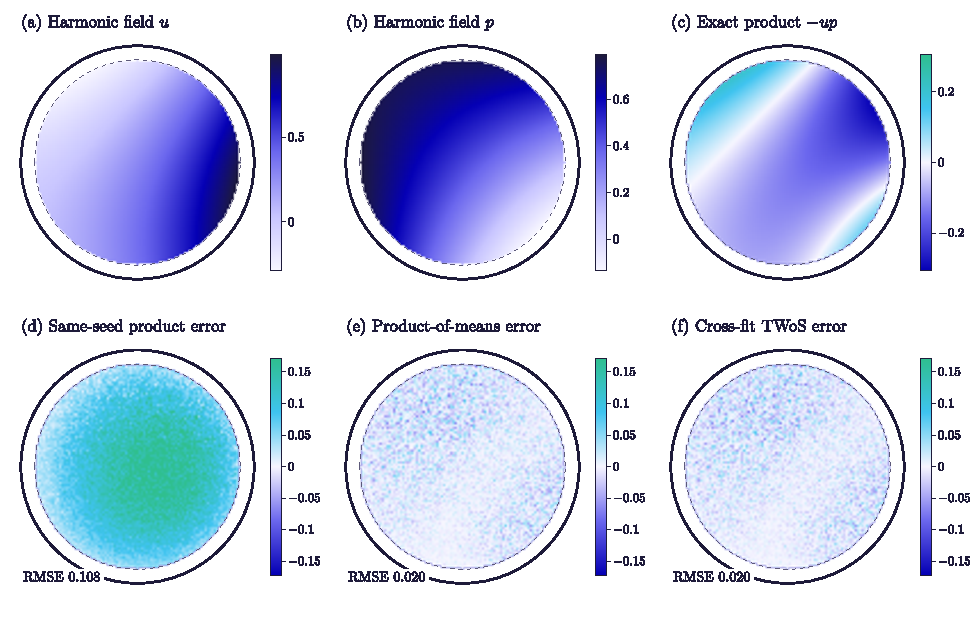
\includegraphics[width=0.96\textwidth]{figures/manufactured-field.pdf}
 \caption{Manufactured spatial validation with actual WoS paths. The two harmonic fields (a--b) and exact product $-up$ (c) supply analytic reference values. Multiplying same-seed primal and adjoint samples creates a coherent covariance-error field (d), with RMSE $0.108$ and mean bias $0.0987$. The product of sample means (e) suppresses the error to RMSE $0.0195$ but retains its finite-$N$ covariance bias. Cross-fitted \method{} (f) has RMSE $0.0196$ and mean bias $-1.20\times10^{-4}$, matching the sampling error while removing the bias exactly in expectation.}
 \label{fig:manufactured}
\end{figure}

\subsection{Three-dimensional internal-cooling reference}

We next exercise scout--rescore--insert placement in three dimensions.
The solid is the box
$[-1.2,1.2]\times[-0.8,0.8]\times[-0.45,0.45]$ with zero-temperature
Dirichlet data on its exterior and on every inserted cooling cavity.  We solve
$-\Delta u=f$ for the positive affine source
$f(x,y,z)=1+0.45x/1.2-0.25y/0.8$ and minimize the thermal compliance
$J=\int_\Omega fu\,dx$.  Since the adjoint equals the state, the normalized
spherical-cavity derivative is $D_T=-u^2$.  Affinity of $f$ makes the source
contribution on every three-dimensional WoS ball exact:
$f(x)R^2/6$.  Both the box and the union of cavities are queried analytically;
the TWoS method therefore constructs no volume grid.

We choose seven cavities of radius $0.115$ among 2,048 scrambled-Sobol
candidate centers, subject to identical exterior and pairwise clearances for
all methods.  Our method uses 16 walks per scouting site, freshly rescores a
24-site shortlist with 192 walks per site, and maximizes the resulting 95\%
lower confidence bound.  We compare against reusing the noisy scout, a
$49\times33\times19$ voxel adjoint/TD solve, and random feasible insertion.
Every design is evaluated on a fixed independent Sobol probe set with fresh
WoS paths; the optimization samples are never reused for the reported
objective.

\begin{figure}[t]
 \centering
 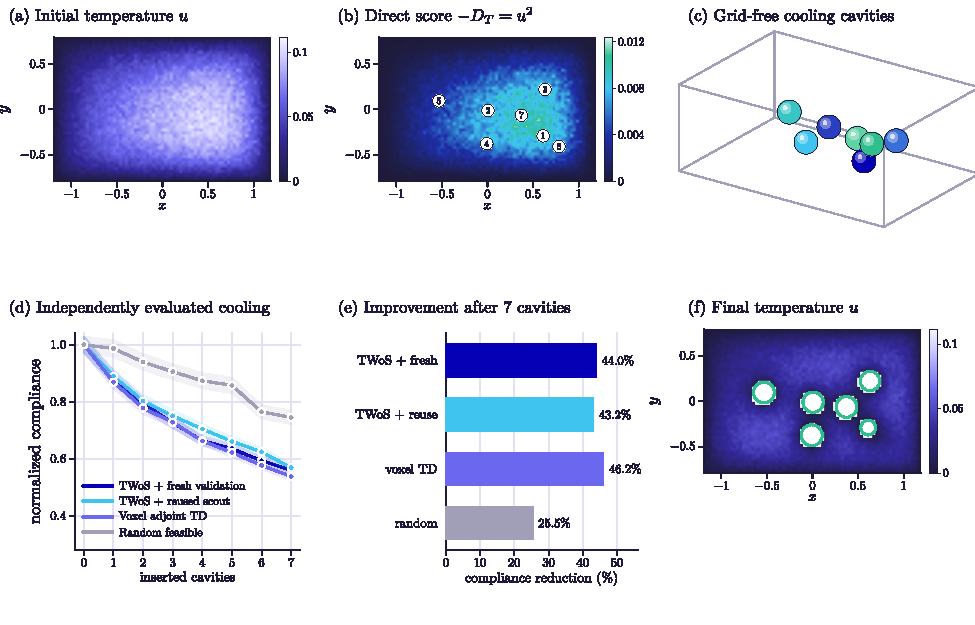
\includegraphics[width=\textwidth]{figures/internal-cooling-benchmark.pdf}
 \caption{Correctness-first 3D internal-cooling benchmark. (a) The initial
 temperature field on the central plane. (b) The direct cross-fitted
 topological score, with selected cavity centers projected onto the plane.
 (c) The resulting grid-free 3D cavity configuration. (d) Independently
 evaluated compliance throughout optimization. (e) Final improvement under
 the same seven-cavity budget. (f) The final central-plane temperature. This
 analytic-geometry pilot validates the complete application loop; it is not
 the final equal-time mesh benchmark.}
 \label{fig:coolingreference}
\end{figure}

The initial TWoS and voxel TD fields have Pearson correlation $0.977$ and
relative RMSE $0.104$.  After seven insertions, validated TWoS reduces
compliance by $43.99\%$, compared with $43.15\%$ for scout reuse, $46.17\%$
for the voxel reference, and $25.47\%$ for random insertion.  Thus the direct
grid-free estimator realizes $95.3\%$ of the voxel baseline's measured
reduction and $1.73\times$ the reduction of random placement.  The small gap
between fresh validation and scout reuse is not statistically resolved in this
single design run; the post-selection coverage experiment in
\cref{fig:controlled}(c), rather than this trajectory, supports the statistical selection mechanism in an idealized known-noise setting. It does not establish finite-cavity coverage for this 3D example.  We likewise withhold a timing claim: the current TWoS
reference is vectorized Python, whereas the sparse voxel solve runs in compiled
code.  The separate compiled Bunny and housing studies measure performance with matched C++ implementations.

\subsection{Stanford Bunny curved-mesh stress test}

The analytic box isolates the optimization mechanism but does not exercise a
production-style curved boundary.  We therefore repeat the complete loop
inside the canonical Stanford Bunny~\cite{stanford1994bunny}.  This experiment
is a geometry stress test, not an engineering claim about cooling a rabbit.
The original zippered reconstruction stores 35,947 vertices and 69,451
triangles and contains five holes in its bottom.  Our deterministic
preprocessing removes 1,113 unreferenced vertices, consistently orients the
faces, seals boundary loops of lengths 22, 42, 39, 40, and 80, and verifies a
closed edge- and vertex-manifold surface with Euler characteristic two.  The
result has 34,839 vertices and 69,674 triangles.

After normalizing the Bunny height to one, we solve the same Poisson-compliance
problem with affine source $f(x,y,z)=1+0.65(y+0.5)$.  We insert six cavities of
radius $0.05$ among 1,024 interior candidate centers.  Exact closest-triangle
distances come from a libigl AABB tree; candidate containment uses fast winding
numbers.  TWoS uses 12 scouting walks and freshly rescores a 20-site shortlist
with 128 walks per site.  The voxel reference uses a
$54\times64\times48$ Cartesian grid clipped by the Bunny.

\begin{figure}[t]
 \centering
 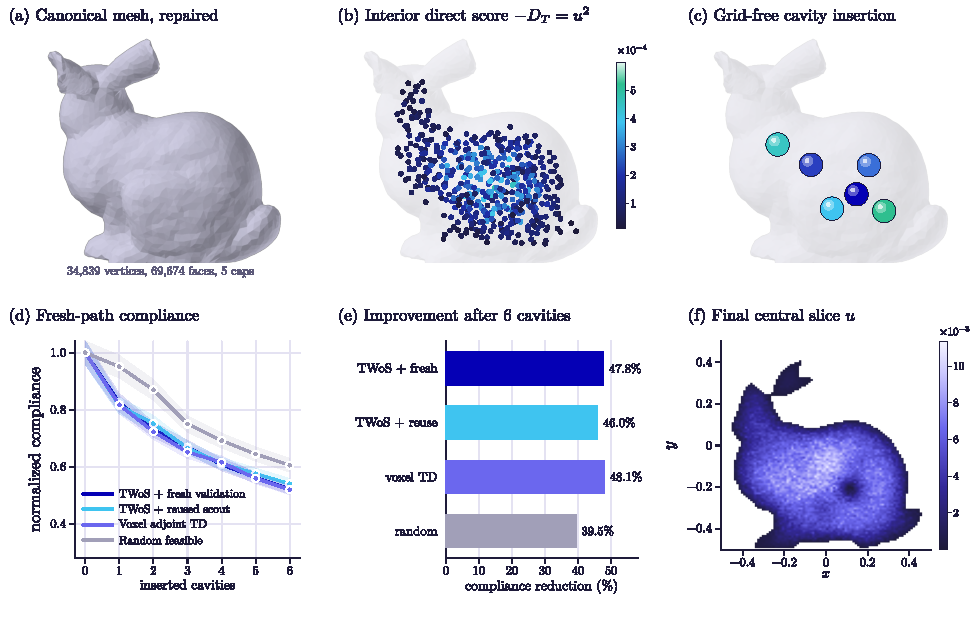
\includegraphics[width=\textwidth]{figures/stanford-bunny-benchmark.pdf}
 \caption{Curved-mesh geometry stress test on the Stanford Bunny. (a) The
 repaired closed input mesh. (b) Interior cross-fitted topological-derivative
 samples viewed through the translucent surface. (c) Six selected cooling
 cavities. (d) Compliance measured with fresh paths after every insertion.
 (e) Improvement under the common cavity budget. (f) Final temperature on the
 central slice. Bunny data courtesy of the Stanford University Computer
 Graphics Laboratory.}
 \label{fig:bunny}
\end{figure}

The noisy 48-walk initial TWoS field has Pearson correlation $0.911$ with the
voxel TD field.  Validated TWoS reduces compliance by $47.77\%$, versus
$45.99\%$ for scout reuse, $48.06\%$ for the voxel reference, and $39.46\%$
for random feasible placement.  It therefore realizes $99.4\%$ of the voxel
reference's reduction without a volume grid; the final-objective point-estimate
gap is smaller than the reported probe-sampling standard errors.  This result
supports geometric applicability; we next isolate field-evaluation performance
with matched compiled implementations.



\subsection{Compiled output-sensitive scaling}

We implemented both methods in the same C++17 executable.  The grid-free kernel
uses Embree~4 closest-point queries and OpenMP over independent paths; the voxel
reference uses the same Embree scene for parity classification, a seven-point
finite-difference stencil, and Eigen conjugate gradients.  Both receive eight
CPU threads.  Timings include BVH construction and all work needed to return the
field, exclude process startup and file I/O, and report the median of three
runs.  Peak resident set size is measured for each isolated process.

We evaluate 384 common interior Sobol sites against an independent
2,048-walk-per-site TWoS reference.  We sweep 4--512 walks per TWoS site and
eight voxel grids from $24\times28\times20$ to $110\times128\times96$.  A
separate output-sensitivity sweep fixes 512 walks per site and a
$96\times112\times84$ grid, which have relative field RMSE $0.0757$ and
$0.0732$, respectively, on all 384 sites, and varies only the requested output
count.

\begin{figure}[t]
 \centering
 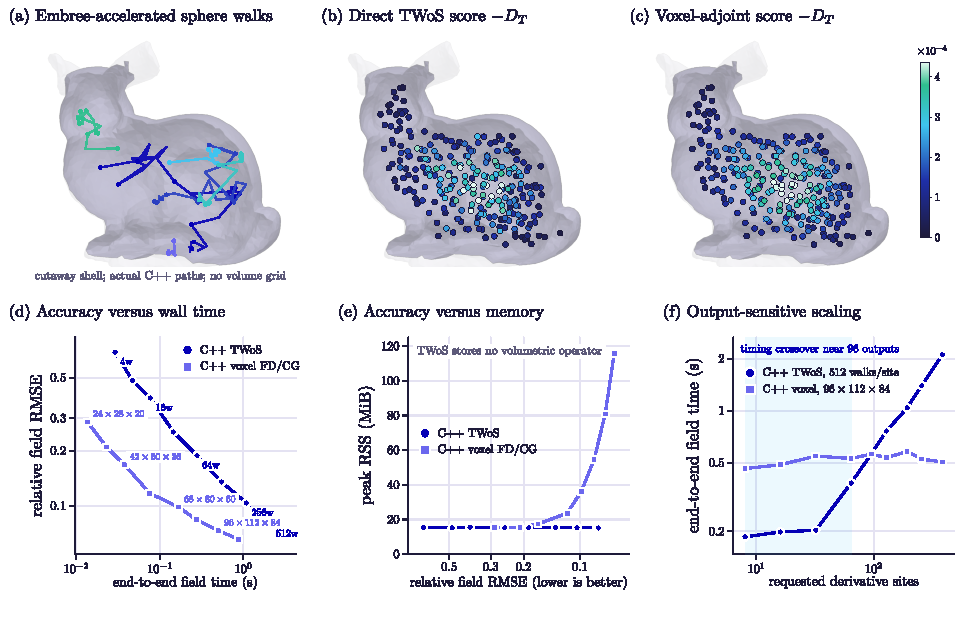
\includegraphics[width=\textwidth]{figures/compiled-bunny-scaling.pdf}
 \caption{Matched C++ scaling on the 69,674-triangle Bunny. (a) Actual
 Embree-accelerated sphere-walk trajectories in a shaded cutaway shell.
 (b--c) Direct TWoS and voxel topological scores at identical exposed interior
 sites and color scale. (d) Relative RMSE
 against an independent 2,048-walk field versus end-to-end time. (e) The same
 accuracy sweep versus measured process peak memory. (f) At nearly matched
 field error, the grid-free method is output-sensitive: the methods tie near
 96 requested sites, and the global voxel solve wins for dense output. Each point
 is measured rather than analytically extrapolated.}
 \label{fig:compiledbunny}
\end{figure}

At 64 outputs, TWoS takes $0.381$ seconds at relative RMSE $0.0622$;
the voxel reference takes $0.528$ seconds at RMSE $0.0711$.  Thus TWoS is
$1.39\times$ faster and its $15.4$ MiB peak is $5.25\times$ smaller than the
voxel process's $80.7$ MiB peak.  The speedup is $2.49\times$ at eight outputs
and the methods are effectively tied at 96 ($0.566$ versus $0.561$ seconds).
At 384 outputs the ordering reverses: TWoS
takes $2.10$ seconds and the voxel solve $0.504$ seconds.  This crossover is the
claimed performance result, not a universal speedup.  In the full-resolution
surface sweep, Embree BVH construction takes $9.74$ ms and the scalar closest-
boundary kernel sustains $1.77$ million queries per second.  Embree distances
agree with libigl to maximum absolute error $3.04\times10^{-7}$; the independent
C++ and Python TWoS fields correlate at $0.991$, and the C++ and SciPy voxel
fields agree to relative RMSE $1.11\times10^{-13}$ at the validation grid.

\paragraph{Independent high-sample check for the teaser.}
\label{app:renderprotocol}
For the 64-site comparison in \cref{fig:teaser}, we recomputed the reference
using an independent seed and 16,384 walks per site. Against this reference,
the retained TWoS and voxel score fields have relative RMSE $0.05888$ and
$0.06886$, respectively. The root-sum-square reference score standard error
divided by the reference score norm is $0.01160$, in addition to error from
the unchanged termination shell $\varepsilon=5\times10^{-4}$. This is a numerical accuracy check,
not exact ground truth; its timing is not included in the performance comparison.
The teaser separately visualizes fresh 256-walk temperature and insertion-benefit
estimates on a $160\times200$ section at $z=0.09$ for the saved cavity designs.
The physical domains do not contain the display opening. A one-grid-cell
Gaussian filter is applied only to the displayed scalar colors; raw fields,
accuracy errors, cooling objectives, and timing data are retained without it.
The placement study and sparse point-query timings are distinct experiments:
the latter does not establish a speedup for the displayed full design loop.

\subsection{Finned-housing design benchmark}

We next test the complete compiled design loop on a license-free stylized
engineering geometry rather than an animal scan.  An analytic union of a
rounded enclosure, nine heat-sink fins, and four mounting bosses is extracted
by marching cubes.  The resulting surface has 48,372 vertices and 96,740
triangles, is connected, closed, edge- and vertex-manifold, and has Euler
characteristic two.  This procedural construction is deliberately auditable;
it resembles a conduction housing but is not proprietary CAD.

Inside the housing we solve $-\Delta u=f$ with zero Dirichlet data on the outer
surface and every inserted cavity.  The positive source is a background plus
three anisotropic Gaussian hot spots representing two chips and a regulator;
the objective is the thermal compliance $J=\int_\Omega fu$.  On each WoS ball,
we sample its Green source integral with the unbiased beta-radial estimator in
\cref{prop:greenballsample}.  Each method inserts six radius-$0.095$ spherical
cavities from the same 768 Sobol candidates.  Sparse \method{} uses 12 scouting
walks per feasible candidate and 192 fresh walks on a 24-site shortlist; a
near-matched-time variant uses 96 and 768 walks, respectively.  Our strongest
deterministic baseline is a matrix-free geometric multigrid solver for the same
embedded seven-point operator, with four levels, three weighted-Jacobi pre- and
post-sweeps, residual-minimizing coarse correction, and relative residual
$10^{-6}$.  A predeclared sweep selects the smallest tested grid whose field
error is at most $0.09$, yielding $113\times73\times57$.  We also retain the
$96\times64\times54$ diagonal-preconditioned FD/CG baseline and random feasible
insertion.

All trajectory objectives use 384 fixed Sobol probes and 160 independent
walks per active probe.  We rerun each stochastic selector end to end for five
independent seeds; every final design is then evaluated with at least five fresh
384-walk streams, while the canonical and deterministic designs use ten.
Error bars for stochastic selectors are standard errors across complete design
runs; deterministic-baseline error bars isolate objective-evaluation noise.
Selection timings include BVH construction and every scouting/validation walk
for \method{}, or hierarchy construction, solve, and interpolation for
multigrid and FD/CG; all exclude process startup, file I/O, and the common
independent objective evaluation.



Across the five complete design runs, sparse and near-matched-time \method{}
reduce compliance by $68.90\%\pm0.84\%$ and $69.39\%\pm0.51\%$, respectively.
Tuned multigrid obtains $70.36\%\pm0.08\%$, FD/CG obtains
$69.96\%\pm0.10\%$, and five random designs obtain $27.76\%\pm4.57\%$.
Thus sparse \method{} realizes $97.9\%$ of the multigrid reduction in $0.432$
seconds rather than $1.861$ seconds, a $4.31\times$ speedup.  At near-matched
time, \method{} realizes $98.6\%$ of the multigrid reduction in $1.731$
seconds and uses $19.1$ MiB peak RSS rather than $31.4$ MiB, a $1.65\times$
memory reduction.  The near-matched-time mean is about one percentage point below multigrid.
The small seed count and the displayed standard errors do not establish
statistical equivalence; we report the quality--cost tradeoff directly.

Relative to a separate 512-walk TWoS field, the initial 128-walk \method{},
multigrid, and FD/CG fields have relative RMSE $0.163$, $0.0852$, and $0.0814$,
respectively.  The multigrid resolution sweep in
\cref{fig:housingtradeoffs}(a) therefore strengthens rather than weakens the
deterministic reference.  The design result does not claim that the inexpensive
scouting map is more accurate: shortlist validation recovers nearly all
multigrid design quality despite noisier global ranking.

\begin{figure}[t]
 \centering
 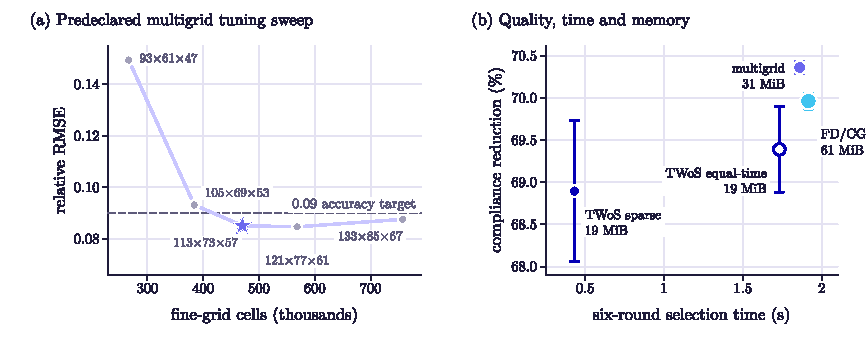
\includegraphics[width=0.89\textwidth]{figures/engineering-housing-tradeoffs.pdf}
 \caption{Tuning and resource tradeoff on the housing benchmark. (a) Five
 multigrid resolutions, each timed three times.  The star is the smallest grid
 meeting the predeclared relative-RMSE target $0.09$ against the independent
 512-walk field.  (b) Final design quality versus complete six-round selection
 time; marker area encodes peak memory and vertical bars show standard errors.
 Sparse \method{} occupies the fast regime, while the near-matched-time budget
 approaches the tuned multigrid solution without allocating a volume grid.}
\label{fig:housingtradeoffs}
\end{figure}

\subsection{Independent tetrahedral FEM audit}

We next remove implementation coupling from the initial-field comparison.  A
separate Python program uses scikit-fem 11.0.0~\cite{gustafsson2020scikitfem}
to assemble continuous piecewise-linear tetrahedra and SciPy's sparse direct
solver.  The only shared inputs are the analytic housing SDF, the analytic
load, and the CSV containing the 768 candidate coordinates; no C++ field,
grid, walk, or interpolation code is reused.  Background tetrahedra are kept
when their centroids lie inside the SDF, all exposed facets receive homogeneous
Dirichlet data, and the reported ranking density is $u_h^2$, since compliance
is self-adjoint for this load case.

We solve at $41\times27\times23$, $61\times39\times33$, and
$81\times51\times43$ background resolutions.  The finest retained mesh has
79,851 vertices and 393,616 tetrahedra; its free-DOF relative algebraic
residual is $5.45\times10^{-14}$.  End-to-end construction, assembly, solve,
and bounded-memory evaluation at all sites takes $20.37$ s and reaches 1.67 GiB
peak RSS in the untuned Python process.  The two coarser fields have relative
RMSE $0.1285$ and $0.0802$ against the finest field, respectively.

\begin{figure}[t]
 \centering
 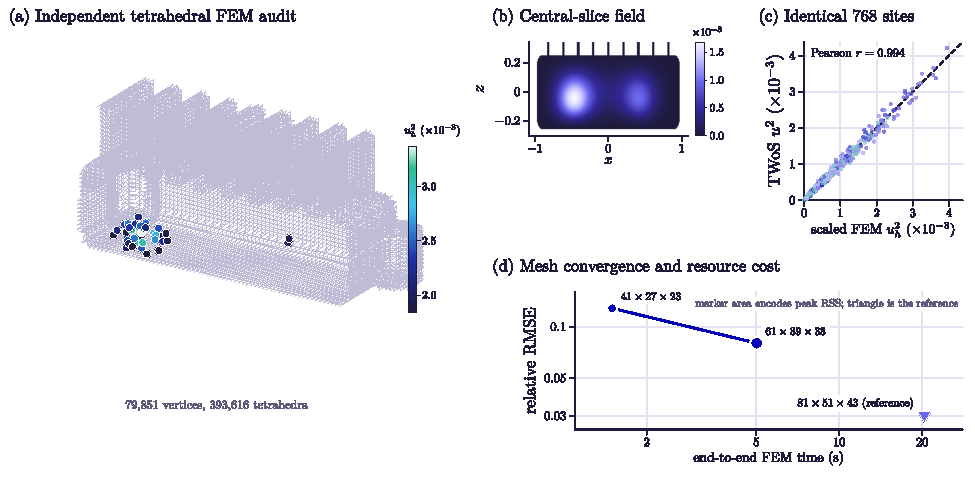
\includegraphics[width=0.92\textwidth]{figures/external-fem-audit.pdf}
 \caption{Independent external-solver field audit. (a) Cutaway boundary facets
 and high-ranking sites on the finest retained tetrahedral mesh. (b) Its
 central-slice $u_h^2$ field. (c) The independently assembled FEM density and
 512-walk TWoS score at the identical 768 candidates after one fitted positive
 scale; color encodes $x$ position. (d) End-to-end time and field convergence
 over three resolutions; marker area encodes measured peak RSS and the triangle
 denotes the finest reference.}
 \label{fig:externalaudit}
\end{figure}

Against the finest FEM field, 128-walk TWoS has Pearson correlation $0.9792$,
Spearman correlation $0.9849$, scale-fitted relative RMSE $0.1514$, and $80\%$
top-20 overlap.  At 512 walks these become $0.9943$, $0.9957$, $0.0789$, and
$95\%$, respectively; top-50 overlap is $92\%$.  The independent check also
supports the in-house reference: the $133\times85\times67$ multigrid field has
Pearson correlation $0.9989$, relative RMSE $0.0416$, and $95\%$ top-20
overlap against FEM.  This experiment validates the field and ranking across
discretization families.  It is not a claim that this centroid-classified mesh
is a production-quality body-fitted discretization, nor a comparison against a
complete level-set FEM optimizer.

\subsection{Connected cooling-channel growth and shape refinement}

The preceding comparison permits six disconnected cavities.  We next impose a
different, practically motivated topology: one connected channel must join two
separated terminals while removing the same nominal volume as the six
radius-$0.095$ spheres.  This constrained result is not compared as a quality
replacement for the unconstrained cavities; the latter remain an informative unconstrained reference, not a proved optimum or upper bound.

We score 3,072 interior Sobol candidates with 48-walk TWoS, select high-score
terminals on opposite sides of the housing, and construct a 24,365-edge
$k$-nearest-neighbor graph.  An edge's Euclidean length is multiplied by a
penalty for low endpoint topological score, and Dijkstra's algorithm supplies
the initial connection.  Resampling and safe smoothing give seven controls.
Fixed segment subdivisions produce a connected union of 22 overlapping balls,
as in \cref{eq:channelparameterization}.  A straight channel between the same
terminals is the geometry-only baseline.

The target removed volume is $0.0215482$.  Every connected trial radius is an
order-statistic calibration on the same $2^{20}$-point Sobol set; all three
reported channels attain QMC volume $0.0215479$, within one quantization bound
from \cref{prop:qmc-volume}.  At each shape round, 4,096 Differential WoS paths
per active probe estimate all 66 center coordinates jointly; the executable
also reports the 22 radius derivatives, hence 88 parameters.  With the explicit
safe-strip test, the six refinement passes take 3.62--3.82 seconds.  The normal
offset is $\ell=0.004$ and the one-offset-width admissible
patch is \cref{eq:channelsafepatch}.  We apply the exact transpose map
in \cref{eq:channelchainrule}, fix the endpoints, smooth the control proposal,
and project out first-order centerline-length change.  Each of the three step
scales uses eight fresh paired 320-walk objective streams.  A one-sided
Student-$t$ upper bound uses a predeclared Bonferroni allocation of $0.05$
across all 18 possible scale tests.  This follows the conditional protocol of
\cref{prop:fresh-shape} under a paired-normal interval assumption; exact
coverage is not established for the sampled differences.  Final values
use eight separate 768-walk streams.

\begin{figure}[t]
 \centering
 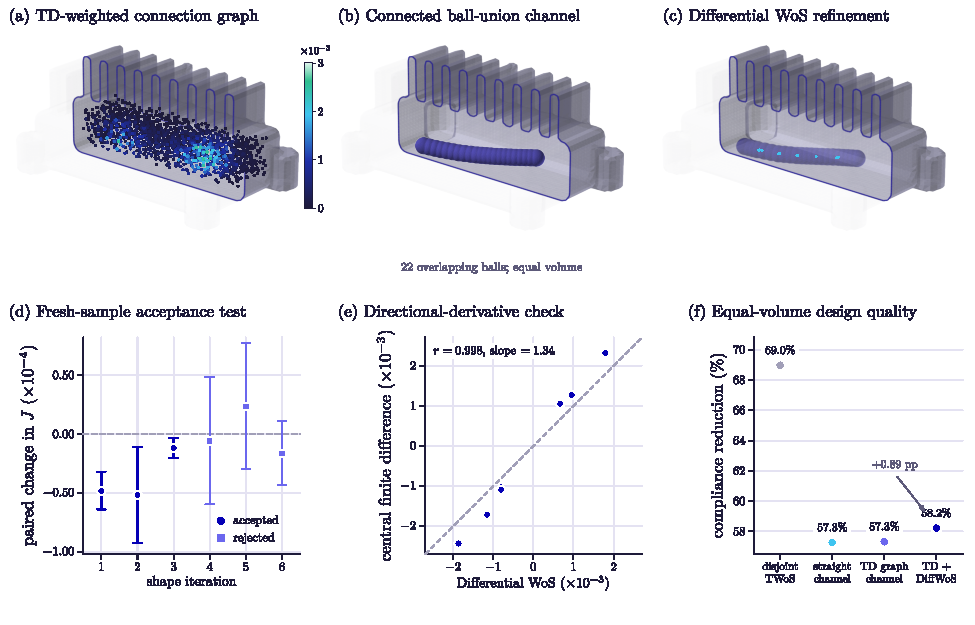
\includegraphics[width=\textwidth]{figures/engineering-housing-channels.pdf}
 \caption{From a topological field to a connected, refined cooling channel.
 (a) A TWoS field selects two terminals and weights the grid-free connection
 graph. (b) The shortest weighted path becomes a 22-ball connected channel.
 (c) Nested Differential WoS moves seven controls; the dashed centerline is
 the pre-refinement path. (d) Fresh paired line-search differences with
 Bonferroni-adjusted Student-$t$ whiskers under the paired-normal model; only a wholly negative interval is
 accepted. (e) Six independent high-signal tangent directions compare the
 fixed-radius Differential WoS derivative with central finite differences.
 (f) Independent final compliance reduction at matched nominal volume. The
 disconnected result is a topology-unconstrained reference, not a connected
 competitor.}
 \label{fig:housingchannels}
\end{figure}

The straight and topology-weighted graph channels reduce compliance by
$57.269\%\pm0.080\%$ and $57.325\%\pm0.048\%$, respectively; their paired
objective difference is not resolved ($-8.60\times10^{-6}\pm1.00\times10^{-5}$
SE).  With safe-strip truncation, the familywise procedure accepts the first
three Differential WoS steps and rejects the remaining tested updates.
Independent evaluation of the accepted shape gives $58.215\%\pm0.037\%$
reduction.  Relative to the unrefined graph channel, the objective decreases by
$2.086\%$; its paired absolute change is
$-1.356\times10^{-4}\pm8.00\times10^{-6}$ SE.  The unconstrained disconnected
design reaches $68.964\%\pm0.050\%$, showing a measured quality gap between these particular constructions; it does not establish the optimal cost of connectivity.

We audit the fixed-radius gradient at the pre-refinement graph channel with an
independent 8,192-walk Differential WoS pass and central differences of step
$0.012$, each using three paired 4,096-walk replicates.  To avoid a
noise-dominated correlation statistic, the predeclared seeded directions are
the descent direction plus five feasible tangent directions spanning the top
30\% of predicted signal; this audit therefore makes no claim about arbitrarily
weak directions.  Across the six signed directions, Pearson correlation is
$0.9982$, cosine similarity is $0.9982$, and the least-squares slope of finite
difference on Differential WoS is $1.341$.  The coherent scale difference is
consistent with finite-offset and finite-difference-step effects in
\cref{prop:channel-diffwos}; signs and relative magnitudes, which drive the
validated line search, agree closely.

\begin{figure}[t]
 \centering
 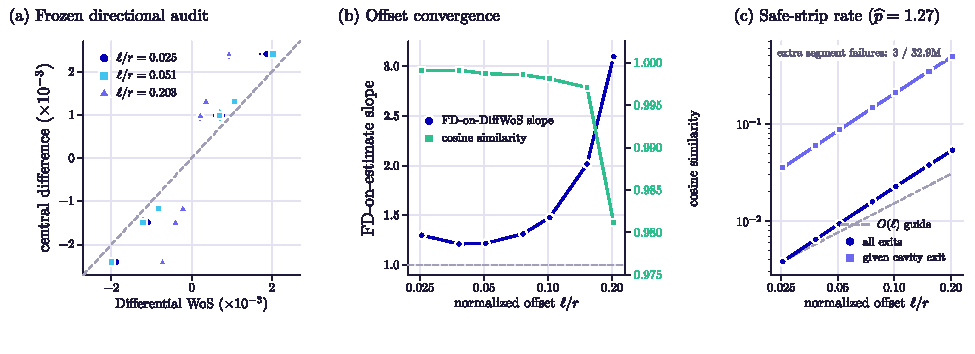
\includegraphics[width=\textwidth]{figures/offset-seam-sweep.pdf}
 \caption{Finite-offset and seam-strip audit on the frozen pre-refinement
 channel. (a) Central finite differences versus Differential WoS for six
 directions selected on a separate pilot stream, shown at the smallest,
 nominal, and largest offsets. (b) FD-on-Differential-WoS slope and cosine
 similarity across all seven normalized offsets. (c) The discarded harmonic
 exit mass, both over all exits and conditional on a cavity exit. The dashed
 line is an $O(\ell)$ reference, while $\widehat p$ is an unconstrained
 log--log fit. Error bars are standard errors over three independent streams;
 the random streams are matched across offsets.}
 \label{fig:offsetseamsweep}
\end{figure}

To isolate the normal offset, we freeze the same seven-control, 22-ball channel
and use an independent 8,192-walk pilot to select six feasible high-signal
length-tangent directions.  The reference central differences use three paired
4,096-walk replicates; each of seven offsets from $0.002$ to $0.016$ then uses
three independent 4,096-walk Differential WoS streams, with seeds matched
across offsets.  All six signs agree at every offset.  Through
$\ell/r=0.102$, cosine similarity is at least $0.9981$; at the deliberately
large $\ell/r=0.203$, it falls to $0.9811$ and the scale-corrected relative
$\ell_2$ error rises to $19.3\%$.  The smallest offset has greater
$1/\ell$ sampling noise: its FD-on-estimate slope is $1.303$, compared with
$1.216$ at $\ell=0.003$.  Linear extrapolation from offsets through $0.008$
has cosine $0.9993$ with the finite differences and FD-on-extrapolate slope
$1.167$; the residual scale difference also includes the finite FD step.

Across 32,858,112 outer paths, the discarded all-exit mass rises from
$0.003874\pm0.000048$ to $0.054123\pm0.000064$.  A log--log fit gives exponent
$1.269$ with $R^2=0.99991$; only three additional normal segments fail the
retained-domain check ($9.13\times10^{-8}$ of paths).  This is strong numerical
evidence for the geometric exit-mass component of
\cref{eq:weightedseamstrip} on this frozen configuration, but it neither
measures the $|\partial_nu|$ weight nor proves the asymptotic hypothesis.

The connected experiment demonstrates compatibility with existing-boundary refinement. Neither the topological graph initialization nor the measured line search supplies an unconditional certificate for the full geometry.

\subsection{Result summary}

\begin{table}[!htbp]
\centering
\caption{Measured results. Controlled diagnostics validate statistical mechanisms; the final rows report matched compiled comparisons, stochastic housing designs, and the equal-volume connected-channel refinement.}
\label{tab:controlledresults}
\begin{tabularx}{\textwidth}{@{}>{\raggedright\arraybackslash}p{0.2\textwidth}>{\raggedright\arraybackslash}p{0.17\textwidth}rr>{\raggedright\arraybackslash}X@{}}
\toprule
Experiment & Metric & Baseline & Ours & Outcome \\
\midrule
Smallest annulus capacity & Variance & $5.83\times10^{-3}$ & $7.06\times10^{-4}$ & $8.26\times$ below coupled finite cavity \\
Correlation $0.9$ & Absolute bias & $2.708\times10^{-1}$ & $7.50\times10^{-4}$ & same-seed error floor removed \\
256 null candidates & False insertion & $100.0\%$ & $5.003\%$ & fresh validation meets 5\% target \\
6,359-site WoS field & Spatial RMSE & $0.1078$ & $0.0196$ & $5.50\times$ below same-seed product \\
64-site C++ field & Wall time (s) & $0.528$ & $0.381$ & $1.39\times$ faster than voxel FD/CG \\
384-site, $\approx0.075$ RMSE & Peak RSS (MiB) & $80.6$ & $15.6$ & $5.17\times$ smaller than voxel FD/CG \\
Housing, sparse budget & Compliance reduction & $70.36\%$ & $68.90\%$ & $97.9\%$ of tuned multigrid reduction \\
Housing, sparse budget & Wall time (s) & $1.861$ & $0.432$ & $4.31\times$ faster than tuned multigrid \\
Housing, near-matched time & Compliance reduction & $70.36\%$ & $69.39\%$ & $98.6\%$ of tuned multigrid reduction \\
Housing, near-matched time & Peak RSS (MiB) & $31.4$ & $19.1$ & $1.65\times$ smaller than tuned multigrid \\
External FEM field audit & Pearson correlation & $1.000$ & $0.9943$ & 512-walk TWoS on identical 768 sites \\
External FEM field audit & Top-20 agreement & $100\%$ & $95\%$ & cross-discretization ranking agreement \\
Connected housing channel & Compliance reduction & $57.325\%$ & $58.215\%$ & $2.086\%$ lower objective after safe-strip DiffWoS refinement \\
Channel derivative audit & Pearson correlation & --- & $0.9982$ & six high-signal tangent directions \\
Channel offset audit & Discarded-mass exponent & $O(\ell)$ reference & $1.269$ & $R^2=0.99991$ over 32.86M paths \\
\bottomrule
\end{tabularx}
\end{table}

